\documentclass[a4paper,12pt]{article}

%================== Núcleo ==================% 
\usepackage[utf8]{inputenc}
\usepackage[T1]{fontenc}
\usepackage[spanish, es-lcroman]{babel}
\decimalpoint
\usepackage{microtype}

% Tipografía y mates
\usepackage{newtxtext,newtxmath}
\usepackage{amsmath,mathtools,bm} 

% Geometría
\usepackage{geometry}
\geometry{
  margin=0.8in,
  headheight=16pt,
  headsep=16pt,
  footskip=16pt
}
\setlength{\parindent}{15pt}
\setlength{\parskip}{0pt}
\usepackage[dvipsnames]{xcolor}
\usepackage{enumitem}
\usepackage{pdflscape}

%================== Colores ==================% 
\usepackage[table]{xcolor} 
\definecolor{lavanda}{HTML}{B8A9C9}
\definecolor{lavandaClaro}{HTML}{F5F2FA}
\definecolor{ink}{HTML}{222222}
\colorlet{Accent}{lavanda}
\colorlet{AccentSoft}{lavandaClaro}
\colorlet{Ink}{ink}

% --- Diagramas con TikZ ---
\usepackage{tikz}
\usetikzlibrary{arrows.meta,positioning,calc,fit}

% Estilos del diagrama
\tikzset{
  human/.style={
    draw=Accent, fill=AccentSoft, rounded corners=4pt,
    minimum width=22mm, minimum height=8mm, line width=0.8pt
  },
  vector/.style={
    draw=Accent, fill=AccentSoft!60, rounded corners=4pt,
    minimum width=22mm, minimum height=8mm, line width=0.8pt
  },
  flow/.style={-Latex, line width=0.9pt, draw=Accent},
  xflow/.style={-Latex, line width=0.9pt, draw=Accent!80},
  aux/.style={dashed, -{Latex[length=2mm]}, draw=Accent!60},
  lab/.style={font=\footnotesize}
}

\usepackage[
  pdfauthor={Debany Jazmín Hernández Camacho},
  pdftitle={Título del artículo},
  colorlinks=true,
  linkcolor=Accent,
  citecolor=Accent,
  urlcolor=Accent
]{hyperref}

% Encabezado / pie
\usepackage{fancyhdr}
\pagestyle{fancy}
\fancyhf{}
\lhead{\footnotesize \textit{Introducción a la Ciencia de Datos}}
\rhead{\footnotesize \textit{Centro de Investigación en Matemáticas - CIMAT}}
\cfoot{\footnotesize \thepage}
\renewcommand{\headrulewidth}{0.6pt}
\makeatletter
\def\headrule{{\color{Accent}\hrule\@height\headrulewidth\@width\headwidth \vskip-\headrulewidth}}
\makeatother

% Títulos
\usepackage{titlesec}
\titleformat{\section}
  {\large\bfseries\color{Ink}}
  {\thesection}{0.6em}
  {\color{Accent}\rule[.5ex]{1.2ex}{1.2ex}\;\;}
\titleformat{\subsection}
  {\normalsize\bfseries\color{Ink}}
  {\thesubsection}{0.6em}
  {\color{Accent}\rule[.5ex]{1ex}{1ex}\;\;}
\titlespacing*{\section}{0pt}{1.1em}{0.6em}
\titlespacing*{\subsection}{0pt}{0.9em}{0.4em}

% Figuras, tablas y leyendas
\usepackage{graphicx}
\usepackage{float}
\usepackage{booktabs}
\usepackage[font=small,labelfont=bf,labelsep=period]{caption}
\usepackage{siunitx}
\sisetup{detect-all,output-decimal-marker={.}}
\graphicspath{{../Figures/}}

%\usepackage[table]{xcolor} 

% Listas
\usepackage{enumitem}
\setlist[itemize]{leftmargin=1.4em}
\setlist[enumerate]{leftmargin=1.6em}

% Cajas discretas
\usepackage[most]{tcolorbox}
\tcbset{boxrule=0.8pt, arc=6pt, left=8pt,right=8pt,top=8pt,bottom=8pt}
\newtcolorbox{abstractbox}{
  enhanced, colback=AccentSoft, colframe=Accent,
  title=\textbf{Resumen}, attach boxed title to top left,
  boxed title style={colback=Accent!20}
}

%================== BibTeX ==================% 
\usepackage[round,authoryear]{natbib}
\bibliographystyle{apalike}

%================== Inicio del documento ==================% 
\begin{document}

\begin{center}
\vspace*{0.5em}
{\LARGE \textbf{\color{Accent}Titulo}\par}
\vspace{0.5em}
{\normalsize Debany Jazmín Hernández Camacho \par}
\vspace{0.25em}
{\footnotesize Centro de Investigación en Matemáticas \;·\; Maestría en Matemáticas Aplicadas \par}
{\footnotesize \texttt{debany.hernandez@cimat.mx} \par}
\vspace{0.8em}
\end{center}

\section{Introducción} La segmentación de clientes es una herramienta fundamental dentro del análisis moderno de datos 
financieros. En particular, las instituciones crediticias requieren identificar patrones de comportamiento que permitan 
distinguir entre individuos con bajo riesgo, perfiles estables y usuarios con una mayor probabilidad de presentar dificultades 
en el pago de sus obligaciones. Esta necesidad surge de la alta heterogeneidad de los clientes: cada persona combina distintos 
niveles de ingreso, uso del crédito, historial de morosidad y carga financiera, lo que hace insuficiente cualquier clasificación 
basada únicamente en una o dos variables. 

En este proyecto se desarrolla un análisis integral de segmentación utilizando el conjunto de datos \textbf{Give Me Some Credit}, 
el cual contiene información financiera y demográfica de aproximadamente 150,000 individuos. El objetivo general es construir 
perfiles homogéneos de clientes a partir de sus características crediticias, sin emplear una variable objetivo o etiquetas previas. 
Para ello se utilizan exclusivamente técnicas de aprendizaje no supervisado, lo que permite dejar que los datos revelen sus 
propias estructuras internas. 

El proceso metodológico combina 3 elementos centrales: 
\begin{itemize}[label=\textcolor{Accent}{$\diamond$}]
  \item una etapa detallada de preprocesamiento para limpiar, imputar y estabilizar las variables, dado que la base de datos 
  presenta altas asimetrías, valores extremos y valores faltantes; 
  \item una reducción de dimensionalidad mediante Análisis de Componentes Principales (PCA), con el fin de capturar la estructura 
  esencial de variabilidad del conjunto; 
  \item un análisis de agrupamiento utilizando K-Means sobre el espacio reducido por PCA. 
\end{itemize}

Más alla del mero cálculo de clusters, el próposito de este estudio es interpretar cada uno de los perfiles resultantes desde una 
perspectiva financiera, buscando responder lo siguiente, ¿qué caracteriza a los clientes menos riesgosos?, ¿qué patrones de 
endeudamiento o morosidad distinguen a los grupos más vulnerables?, ¿cómo se relacionan variables como ingresos, utilización de 
crédito y número de dependientes con el comportamiento crediticio? El énfasis está puesto en describir estos perfiles de forma 
clara y útil, de modo que el agrupamiento tenga un sentido práctico dentro del contexto del riesgo financiero. 

Así, este trabajo no solo construye una segmentación estadísticamente coherente, sino que busca comprender qué factores dan 
forma a los distintos tipos de clientes. El resultado es un análisis que combina técnica, interpretación y una visión aplicada 
de la Ciencia de Datos dentro del ámbito del endeudamiento personal. 

\section{Exploración inicial de los datos}
El análisis se basa en el conjunto de datos \textit{Give Me Some Credit}, el cual contiene información financiera y demográfica 
a nivel individual. Cada fila corresponde a un cliente distinto y resume su situación creditica en un momento específico, a 
partir de un conjunto de variables cuantitativas relacionadas con ingreso, endeudamiento, uso del crédito y comportamiento 
de pago. Para este trabajo se utiliza la versión depurada del archivo \texttt{cs\_training.csv}, que incluye aproximadamente 
150,000 observaciones. Todas las variables empleadas en el análisis son numéricas, lo que facilita el uso de técnicas de reducción 
de dimensionalidad y agrupamiento basadas en distancias. La estructura general del conjunto puede verse como una matriz de tamaño 
$n \times p$, donde $n$ es el número de clientes y $p$ el número de variables consideradas. 

La base de datos original contiene una variable binaria asociada a morosidad severa a dos años (\texttt{SeriousDlqin2yrs}), así 
como diez predictores numéricos que describen hábitos de uso del crédito, niveles de deuda, historial de atrasos y características
demográficas simples (edad y número de dependientes). En este proyecto, dicha variable binaria se utiliza únicamente como información
contextual y no forma parte del proceso de agrupamiento, que se construye de manera completamente no supervisada. 

En la Tabla~\ref{tab:variables} se resumen las variables principales utilizadas, indicando para cada una su tipo de dato y una 
breve descripción de su significado dentro del contexto financiero del problema. 

\begin{table}[H]
\centering
\rowcolors{2}{lavandaClaro!40}{white}
\caption{\textbf{Descripción de las variables de la base de datos}}
\label{tab:variables}
\small
\begin{tabular}{p{5cm} p{3 cm} p{7.5cm}}
\toprule
\rowcolor{lavanda!30}
\textbf{Variable} & \textbf{Tipo} & \textbf{Descripción} \\
\midrule

\texttt{SeriousDlqin2yrs} & Binaria (0/1) &
Indica si el cliente incurrió en morosidad grave (90+ días de atraso) en los próximos dos años. \\

\texttt{RevolvingUtilizationOfUnsecuredLines} & Numérica continua ($\ge 0$) & Proporción de utilización 
de las líneas de crédito no aseguradas (por ejemplo, tarjetas de crédito). Valores cercanos a 1 
indican uso al límite. \\

\texttt{age} & Numérica discreta &
Edad del cliente en años. \\

\texttt{NumberOfTime30-59DaysPastDueNotWorse} & Numérica discreta ($\ge 0$) &
Número de veces con atrasos de 30--59 días, sin caer en morosidad severa. \\

\texttt{DebtRatio} & Numérica continua ($\ge 0$) &
Razón entre el total de pagos mensuales de deuda y gastos, respecto al ingreso mensual declarado. Mide la carga financiera 
relativa del cliente. \\

\texttt{MonthlyIncome} & Numérica continua ($\ge 0$) &
Ingreso mensual declarado por el cliente. \\

\texttt{NumberOfOpenCreditLinesAndLoans} & Numérica discreta ($\ge 0$) &
Número de líneas de crédito y préstamos abiertos (tarjetas, préstamos personales, etc.). \\

\texttt{NumberOfTimes90DaysLate} & Numérica discreta ($\ge 0$) &
Número de atrasos de 90 días o más. Indicador de morosidad severa. \\

\texttt{NumberRealEstateLoansOrLines} & Numérica discreta ($\ge 0$) &
Número de préstamos inmobiliarios (por ejemplo, hipotecas). \\

\texttt{NumberOfTime60-89DaysPastDueNotWorse} & Numérica discreta ($\ge 0$) &
Número de veces que el cliente ha estado entre 60--89 días de atraso, sin caer en estados peores. \\

\texttt{NumberOfDependents} & Numérica discreta ($\ge 0$) &
Cantidad de dependientes económicos del cliente. \\

\bottomrule
\end{tabular}
\end{table}

\section{Metodología}

En esta etapa, el análisis se desarrolló siguiendo un flujo de trabajo estructurado que permite 
transformar la base de datos original en una representación más estable y útil para descubrir 
patrones. Dado que la información financiera suele presentar irregularidades importantes, distribuciones 
muy sesgadas, outliers y escalas poco comparables, el primer paso consistió en preparar 
cuidadosamente las variables para asegurar que todas aportaran de manera equilibrada al modelo.

Una vez obtenidos los datos en condiciones adecuadas, se aplicó una reducción de dimensionalidad 
mediante Análisis de Componentes Principales (PCA), con el fin de concentrar la mayor parte de la 
variabilidad del conjunto en unas cuantas dimensiones interpretables. Este espacio reducido facilita 
tanto la visualización como la separación de los individuos en grupos más homogéneos.

Finalmente, sobre la representación generada por PCA se llevó a cabo un proceso de agrupamiento no 
supervisado mediante K-Means, buscando identificar perfiles de clientes con características 
financieras similares. Las etapas que siguen describen con detalle cada una de estas fases: desde el 
preprocesamiento hasta la construcción de los clusters finales.


\subsection{Preprocesamiento}
El preprocesamiento fue una etapa esencial debido a la presencia de outliers, datos faltantes y distribuciones altamente 
asimétricas, todas características comunes en información financiera. El objetivo de esta fue obtener un conjunto de datos 
estable, consistente y adecuado para la aplicación de técnicas basadas en distancia, especialmente PCA y K-Means. 

En primer lugar, se eliminaron los registros duplicados y un único caso con edad igual a 0, valor imposible en el contexto de 
estudio. Posteriormente, se atendieron los valores faltantes: \texttt{MonthlyIncome} presentaba aproximadamente 5,400 
observaciones vacías, que fueron imputadas mediante la mediana de la distribución, una estrategia adecuada dada su fuerte asimetría. 
Para \texttt{NumberOfDependents} se empleó la moda, pues la mayoría de los clientes declara entre cero y dos dependientes. 

Antes de aplicar transformaciones adicionales, se examinó la matriz de correlación de las variables financieras. Esta permitió 
identificar que, si bien existen asociaciones relevantes entre ciertos pares por ejemplo, entre las distintas medidas de morosidad o 
entre el nivel de ingreso y la actividad crediticia, muchas de las correlaciones son de magnitud moderada o baja. Esta estructura 
sugiere que las variables capturan dimensiones distintas del comportamiento financiero y que ninguna domina por completo a las demás. 
El patrón observado respalda el uso de una técnica de reducción de dimensionalidad como PCA, capaz de sintetizar información dispersa 
en múltiples sentidos de variación.

\begin{figure}[H]
    \centering
    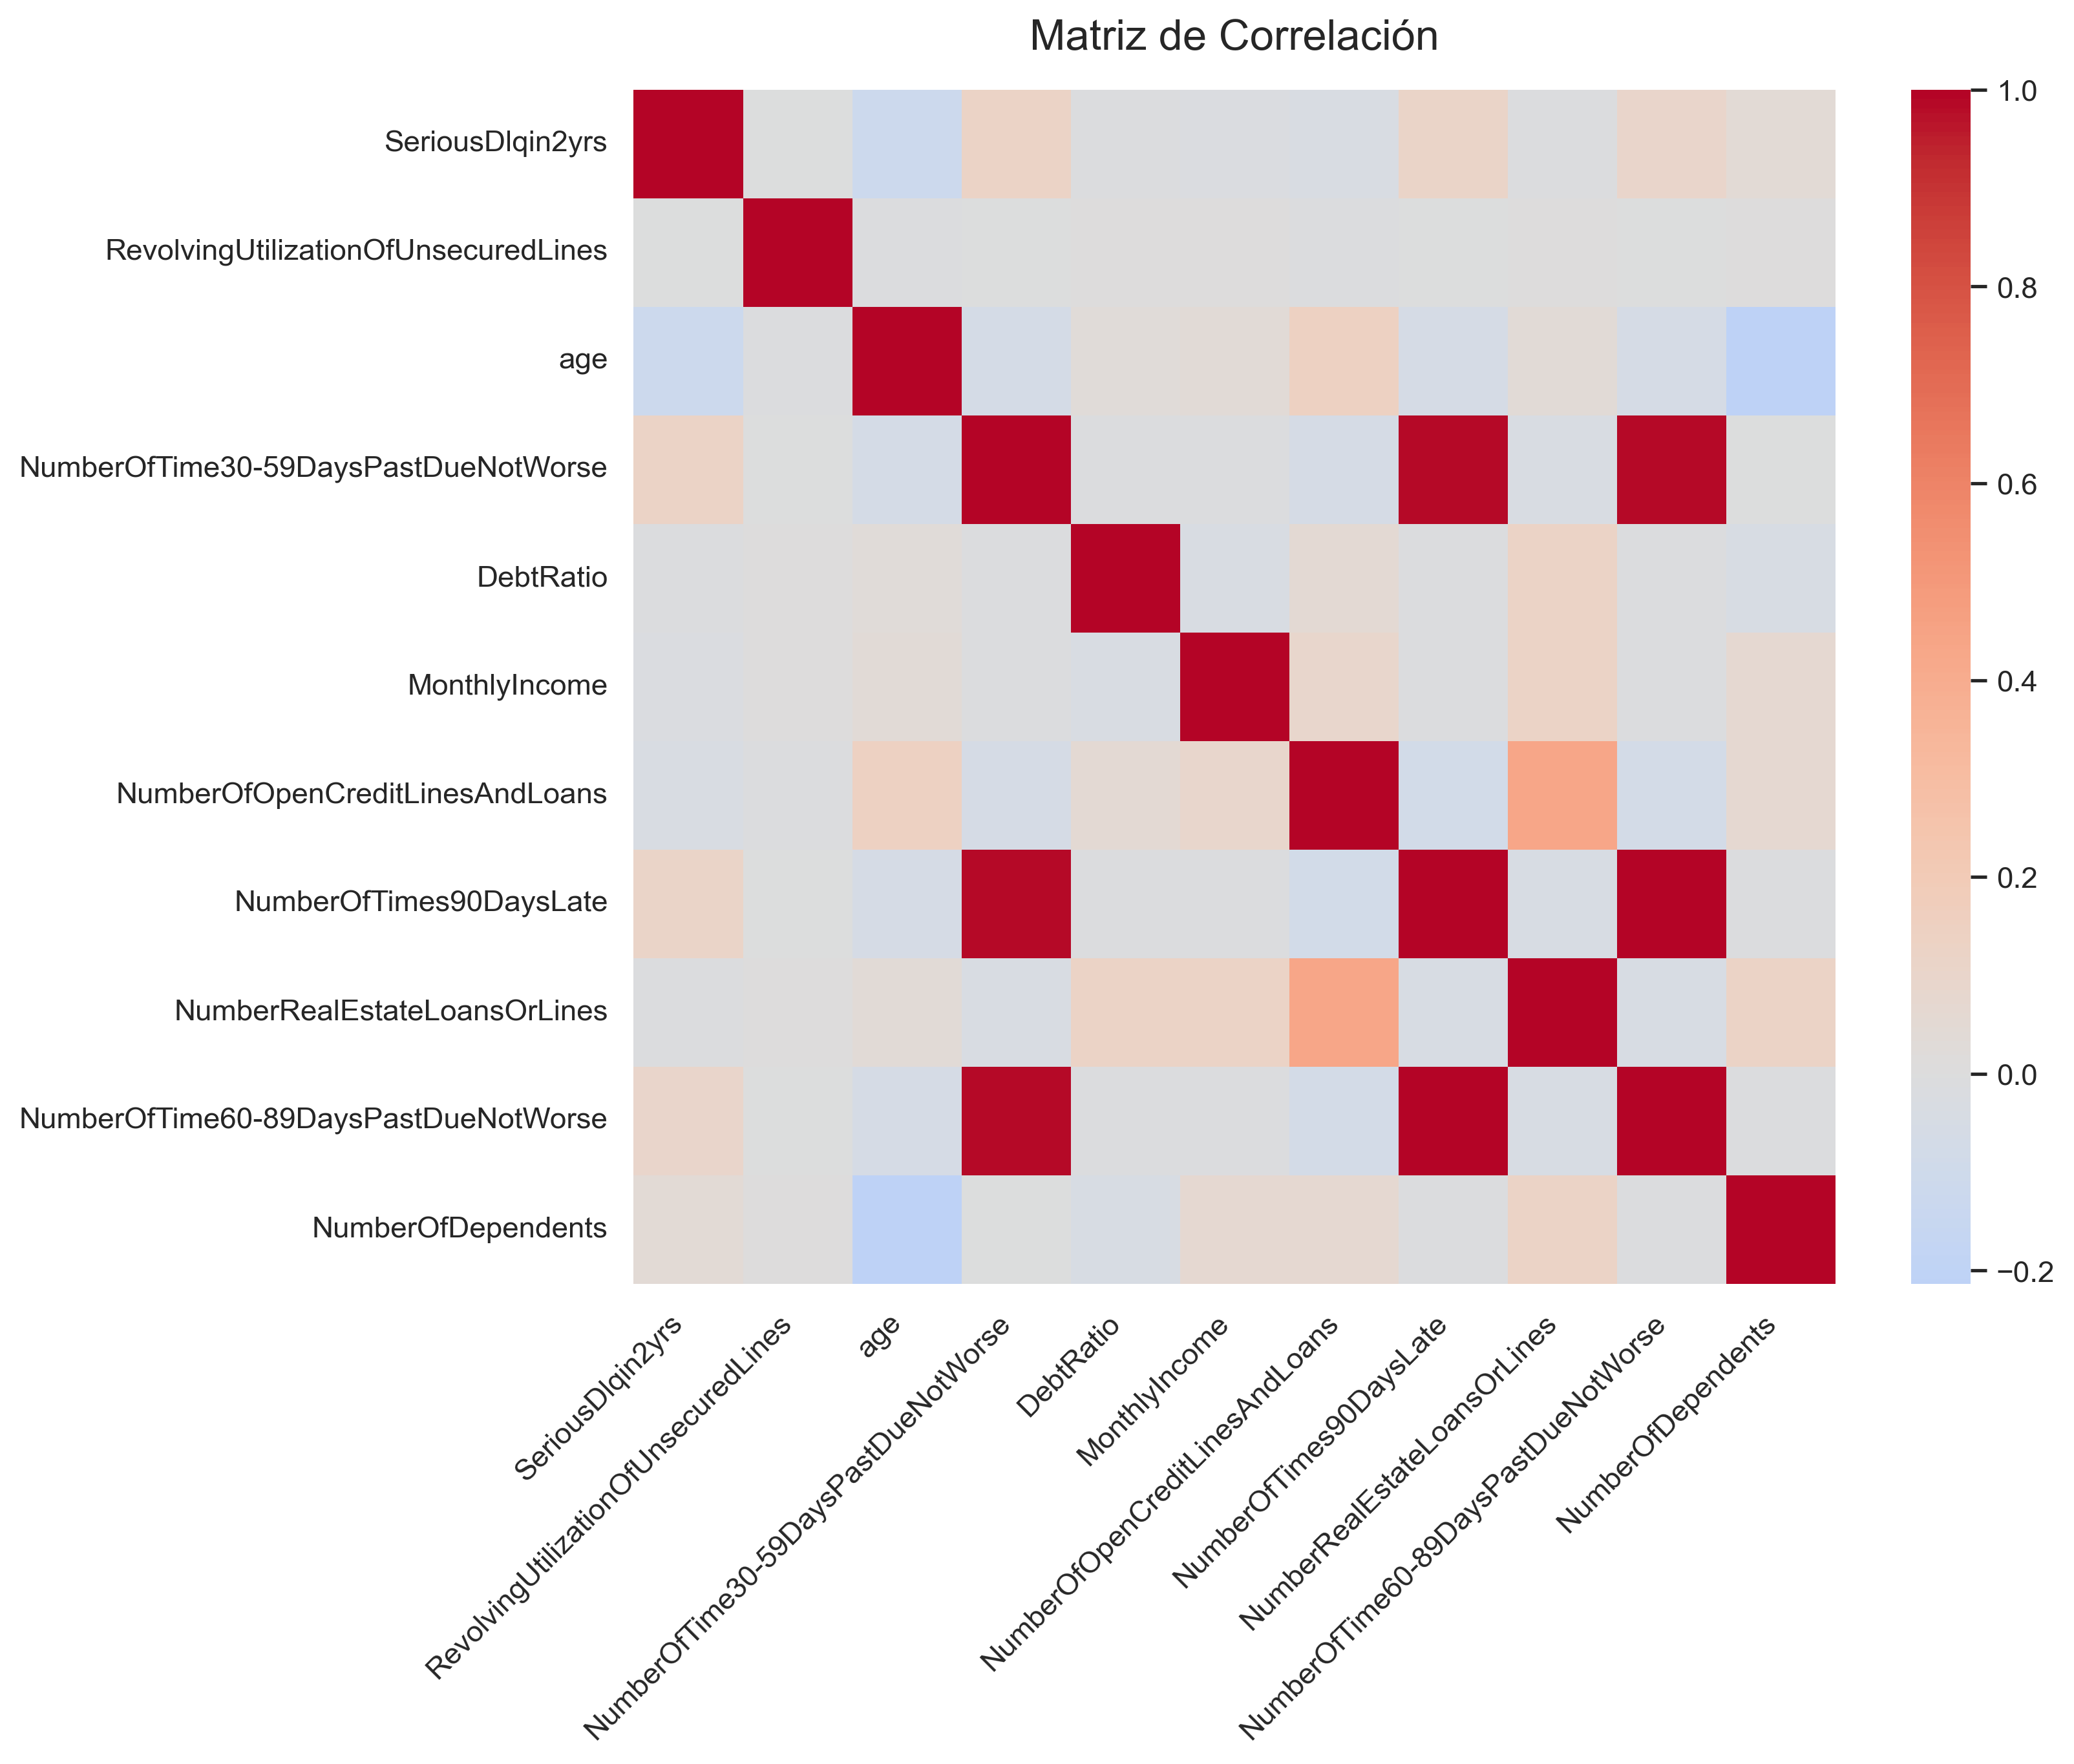
\includegraphics[width=0.7
    \textwidth]{matriz_correlacion.png}
    \caption{Matriz de correlación del conjunto de variables financieras.}
\end{figure}

Un análisis exploratorio reveló la existencia de valores extremadamente grandes en variables como 
\texttt{RevolvingUtilizationOfUnsecuredLines} y \texttt{DebtRatio}. Estos valores, aunque plausibles en ciertos contextos de 
endeudamiento, afectan de manera desproporcionada a métodos sensibles a la escala. Para controlar este efecto sin eliminar 
observaciones completas, se aplicó "winsorización": \texttt{RevolvingUtilizationOfUnsecuredLines} fue truncada en su percentil 99, 
mientras que \texttt{DebtRatio} se truncó en el percentil 99.5 debido a la presencia de outliers particularmente severos. 

Una vez estabilizadas las distribuciones, todas las variables fueron estandarizadas mediante \textit{StandarScaler}. Esta normalización
garantiza que cada variable contribuya en igualdad de condiciones al análisis, evitando que aquellas con rangos grandes dominen los 
componentes principales o los centroides del clustering. El resultado final de esta etapa fue un conjunto limpio, sin valores 
faltantes, con outliers suavizados y todas las variables expresadas en una escala comparable. 


\subsection{Reducción de dimensionalidad mediante PCA}

Una vez que las variables estuvieron depuradas y estandarizadas, se aplicó un Análisis de Componentes Principales (PCA) con 
el objetivo de sintetizar la información esencial del conjunto en un número reducido de dimensiones. 
Esta técnica permite identificar combinaciones lineales de las variables originales que concentran la mayor parte de la 
variabilidad total, lo cual resulta especialmente útil cuando se trabaja con datos altamente correlacionados o con estructuras 
difíciles de visualizar directamente.

El PCA se estimó inicialmente sin fijar un número específico de componentes, permitiendo analizar la proporción de varianza 
capturada por cada dirección principal. La Figura~\ref{fig:varianza-pca} muestra tanto la varianza explicada individual como 
la acumulada. A partir de este análisis, se observó que los primeros seis componentes concentran aproximadamente el 87.6\% de 
la variabilidad total, proporción suficiente para conservar la estructura global de los datos sin incluir dimensiones dominadas 
por ruido o fluctuaciones menores. En consecuencia, el análisis posterior se realizó únicamente sobre este espacio reducido de 
seis dimensiones.

\begin{figure}[H]
    \centering
    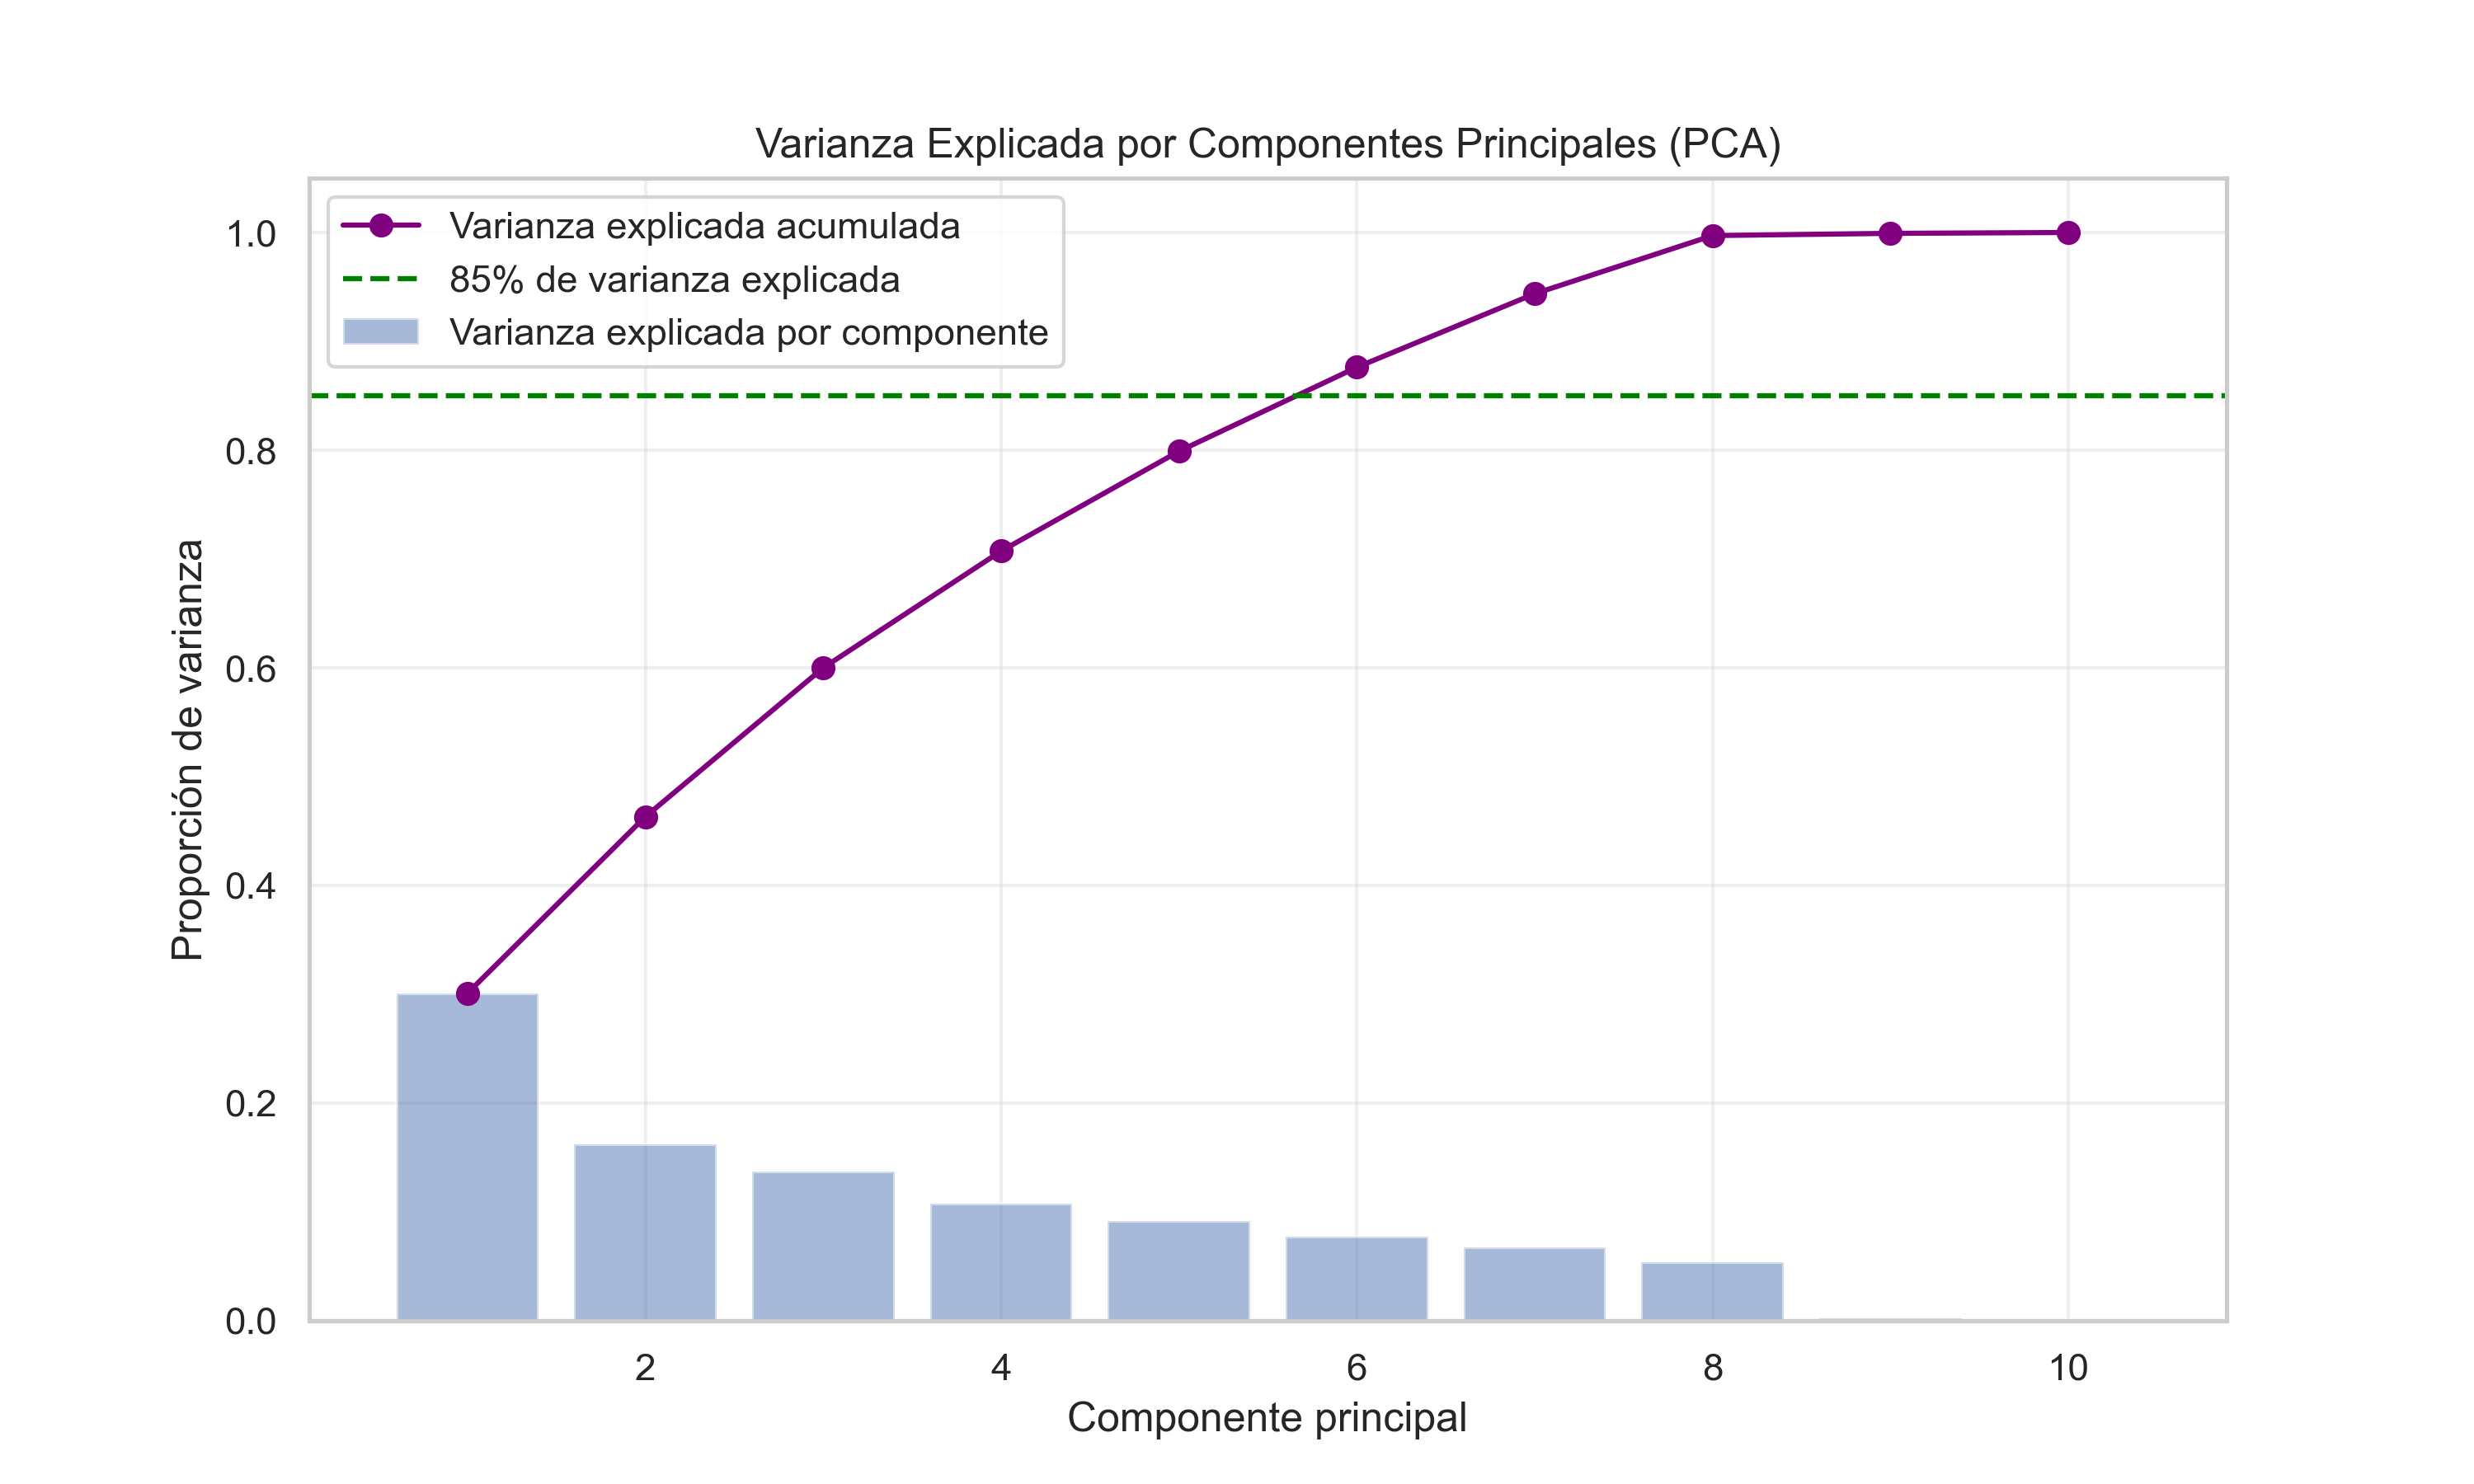
\includegraphics[width=0.95\textwidth]{varianza_explicada_pca.png}
    \caption{Varianza explicada por cada componente principal y varianza acumulada.}
    \label{fig:varianza-pca}
\end{figure}

Además de la reducción en la complejidad, el PCA facilita una interpretación cualitativa de los patrones subyacentes. 
El examen de los \textit{loadings} mostró que ciertos componentes están fuertemente asociados al nivel general de endeudamiento, mientras 
que otros reflejan principalmente la morosidad, la actividad crediticia o la capacidad económica. Estas relaciones permiten entender 
qué factores impulsan las diferencias entre los individuos y proporcionan un marco interpretativo sólido para el paso final 
de agrupamiento.

En conjunto, el uso de PCA no solo mejora la estabilidad del modelo de clustering, sino que también aporta una representación 
más clara y manejable de la estructura del conjunto de datos.

\subsection{Construcción del modelo de agrupamiento}

Una vez definido el espacio reducido mediante PCA, el siguiente paso fue construir el modelo de agrupamiento sobre las seis 
componentes principales. Para decidir cuántos grupos utilizar, se evaluaron distintos valores de $k$ en el rango de 2 a 10 
aplicando el algoritmo K-Means sobre el DataFrame transformado (\texttt{df\_pca}). Para cada valor de $k$ se calcularon 
dos cantidades: la inercia (suma de distancias cuadráticas de cada punto a su centroide) y el coeficiente de Silhouette asociado 
a la partición obtenida.

La Figura~\ref{fig:elbow-kmeans} muestra el comportamiento de la inercia en función de $k$. Como es de esperarse, la inercia 
disminuye de manera monótona al aumentar el número de clusters, pero la tasa de descenso no es constante. Se observa una 
caída pronunciada entre $k = 2$ y $k \approx 4$–$6$, seguida de una zona donde la curva se aplana. Este “codo” sugiere que 
a partir de cinco grupos los beneficios de seguir aumentando $k$ son marginales en términos de reducción de inercia.

\begin{figure}[H]
    \centering
    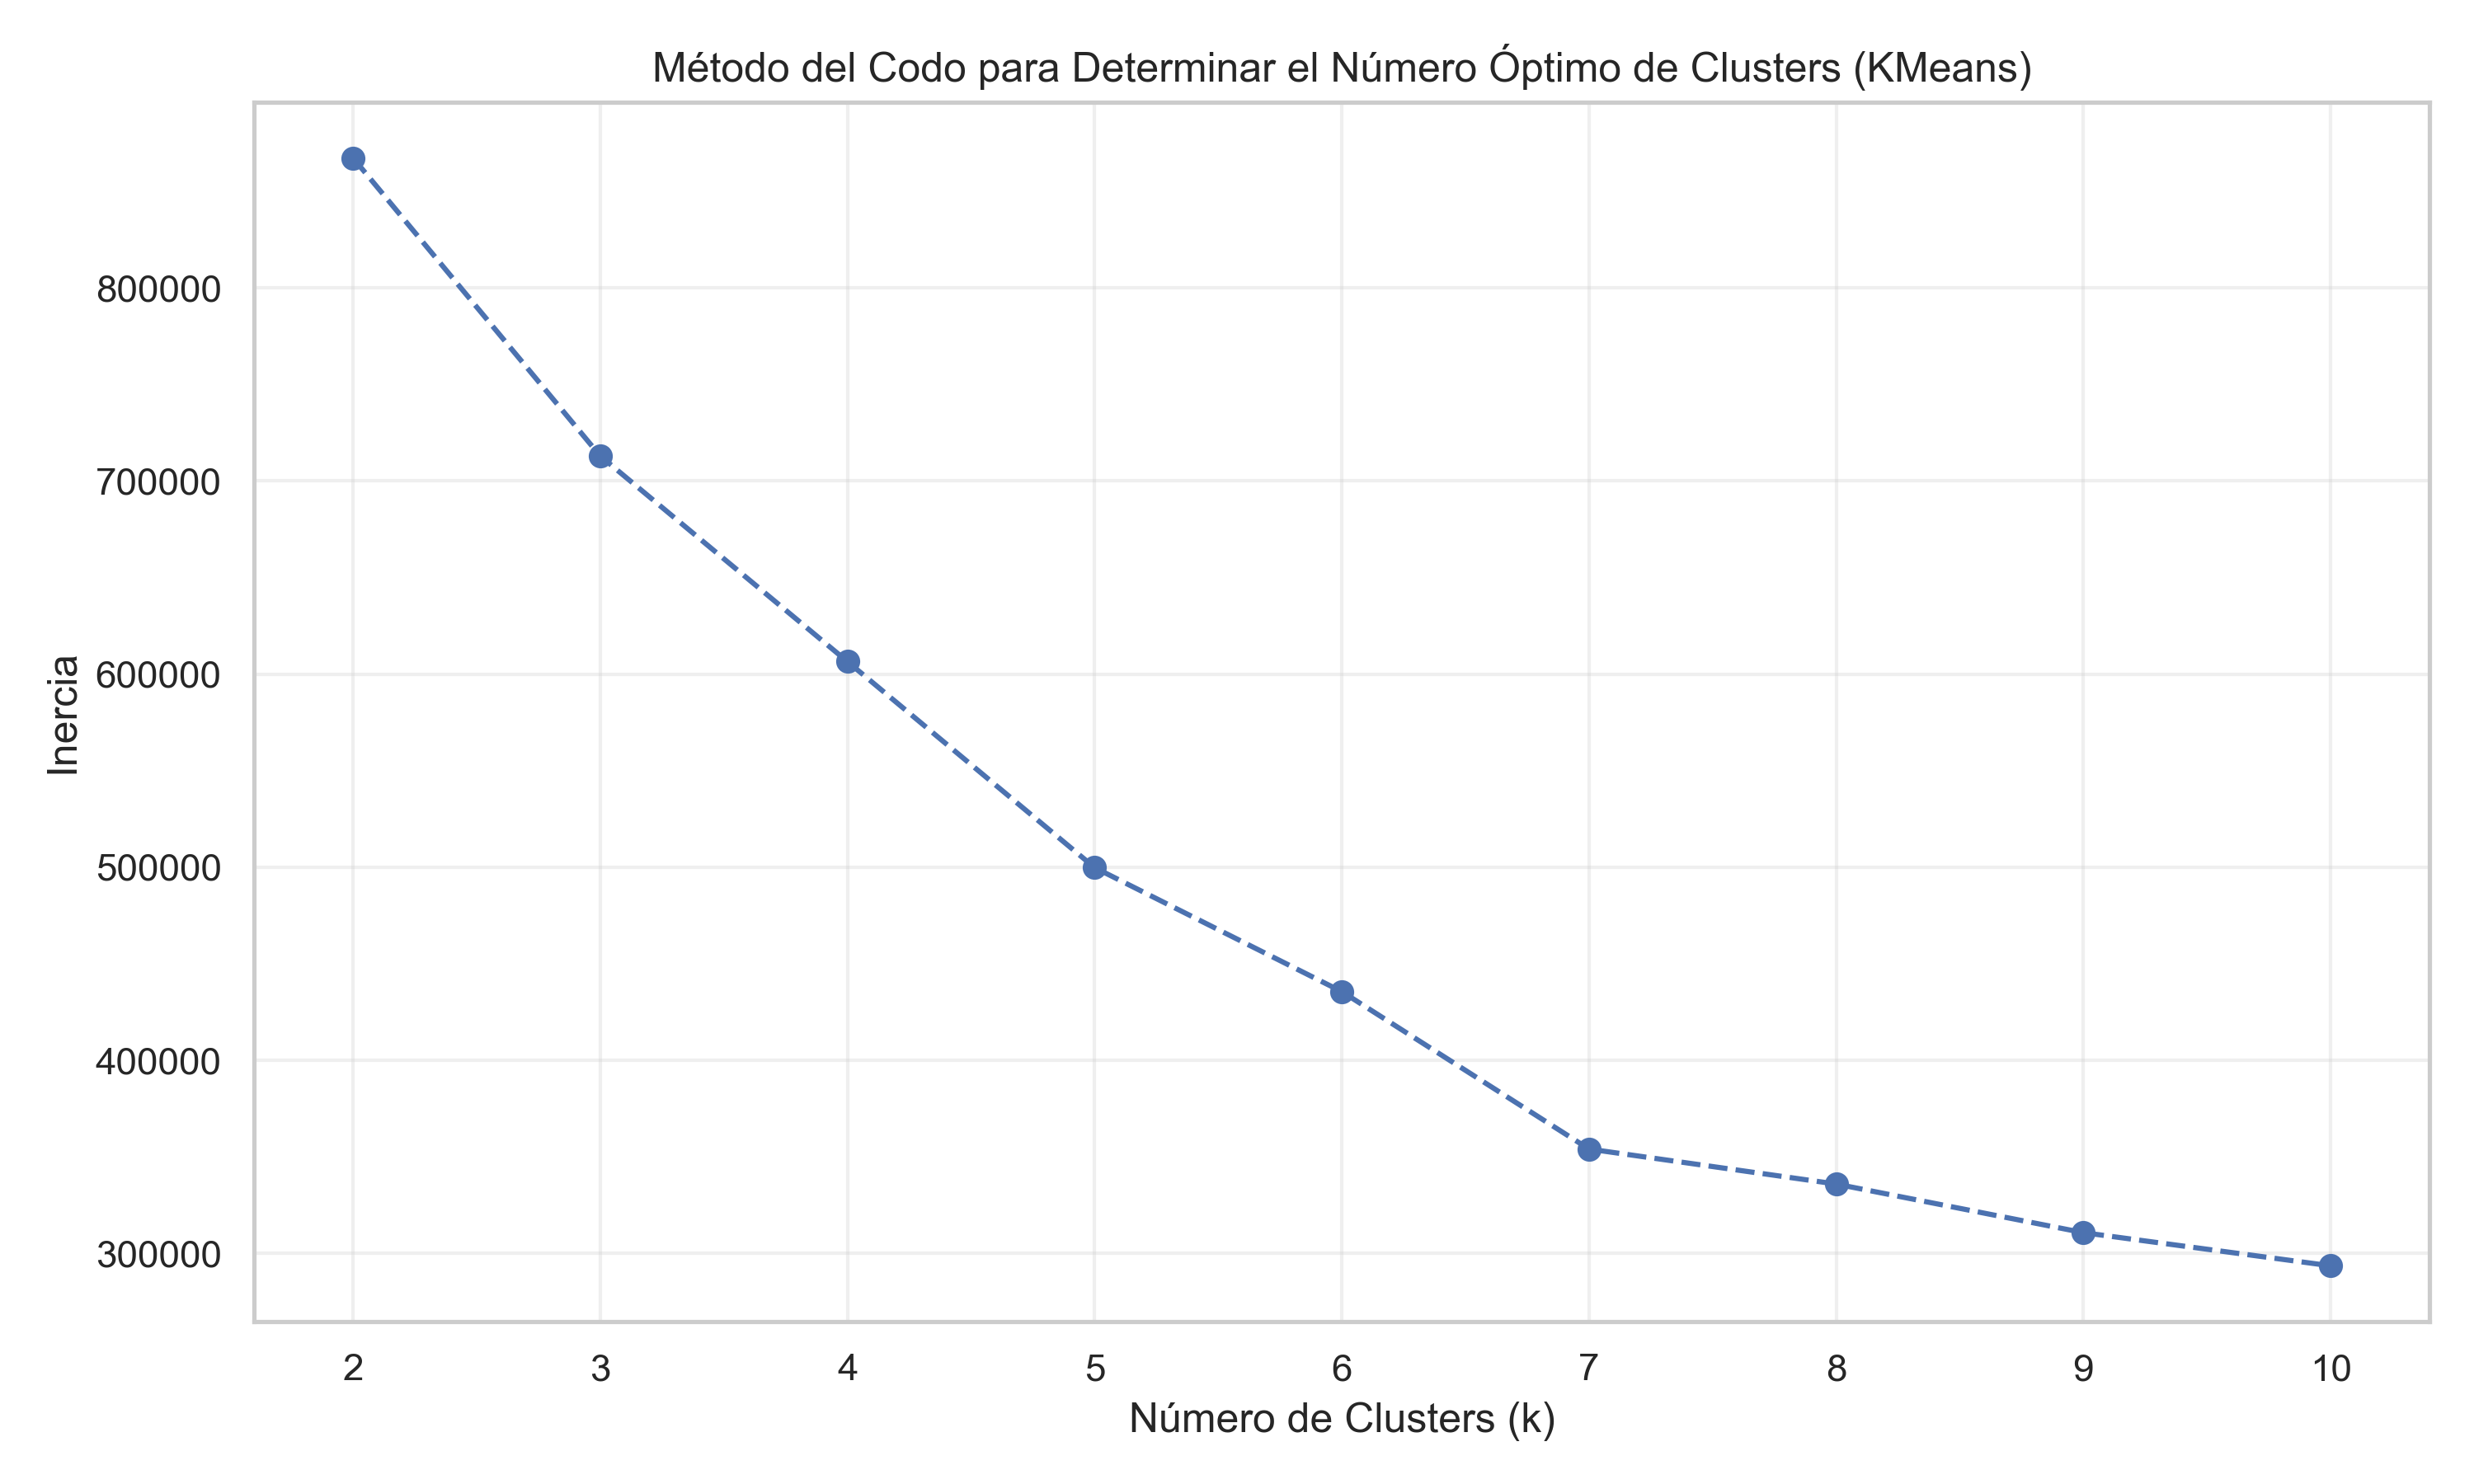
\includegraphics[width=0.87\textwidth]{metodo_del_codo_kmeans.png}
    \caption{Método del codo para distintos valores de $k$ en el modelo K-Means.}
    \label{fig:elbow-kmeans}
\end{figure}

De manera complementaria, la Figura~\ref{fig:silhouette} muestra el coeficiente de Silhouette promedio para los 
mismos valores de $k$. El valor más alto se obtiene en $k = 2$, lo que refleja una separación muy marcada entre dos 
grandes grupos de individuos. Sin embargo, a partir de $k = 3$ los valores de Silhouette se estabilizan en un rango 
cercano a $0.25$–$0.30$, indicando que es posible considerar particiones más finas sin perder coherencia en la separación 
entre clusters. En particular, los valores alcanzados para $k = 5$ son comparables a los de otros modelos con $k > 2$, 
pero permiten distinguir matices adicionales en los patrones de endeudamiento y morosidad que quedarían ocultos en una 
segmentación demasiado gruesa.

\begin{figure}[H]
    \centering
    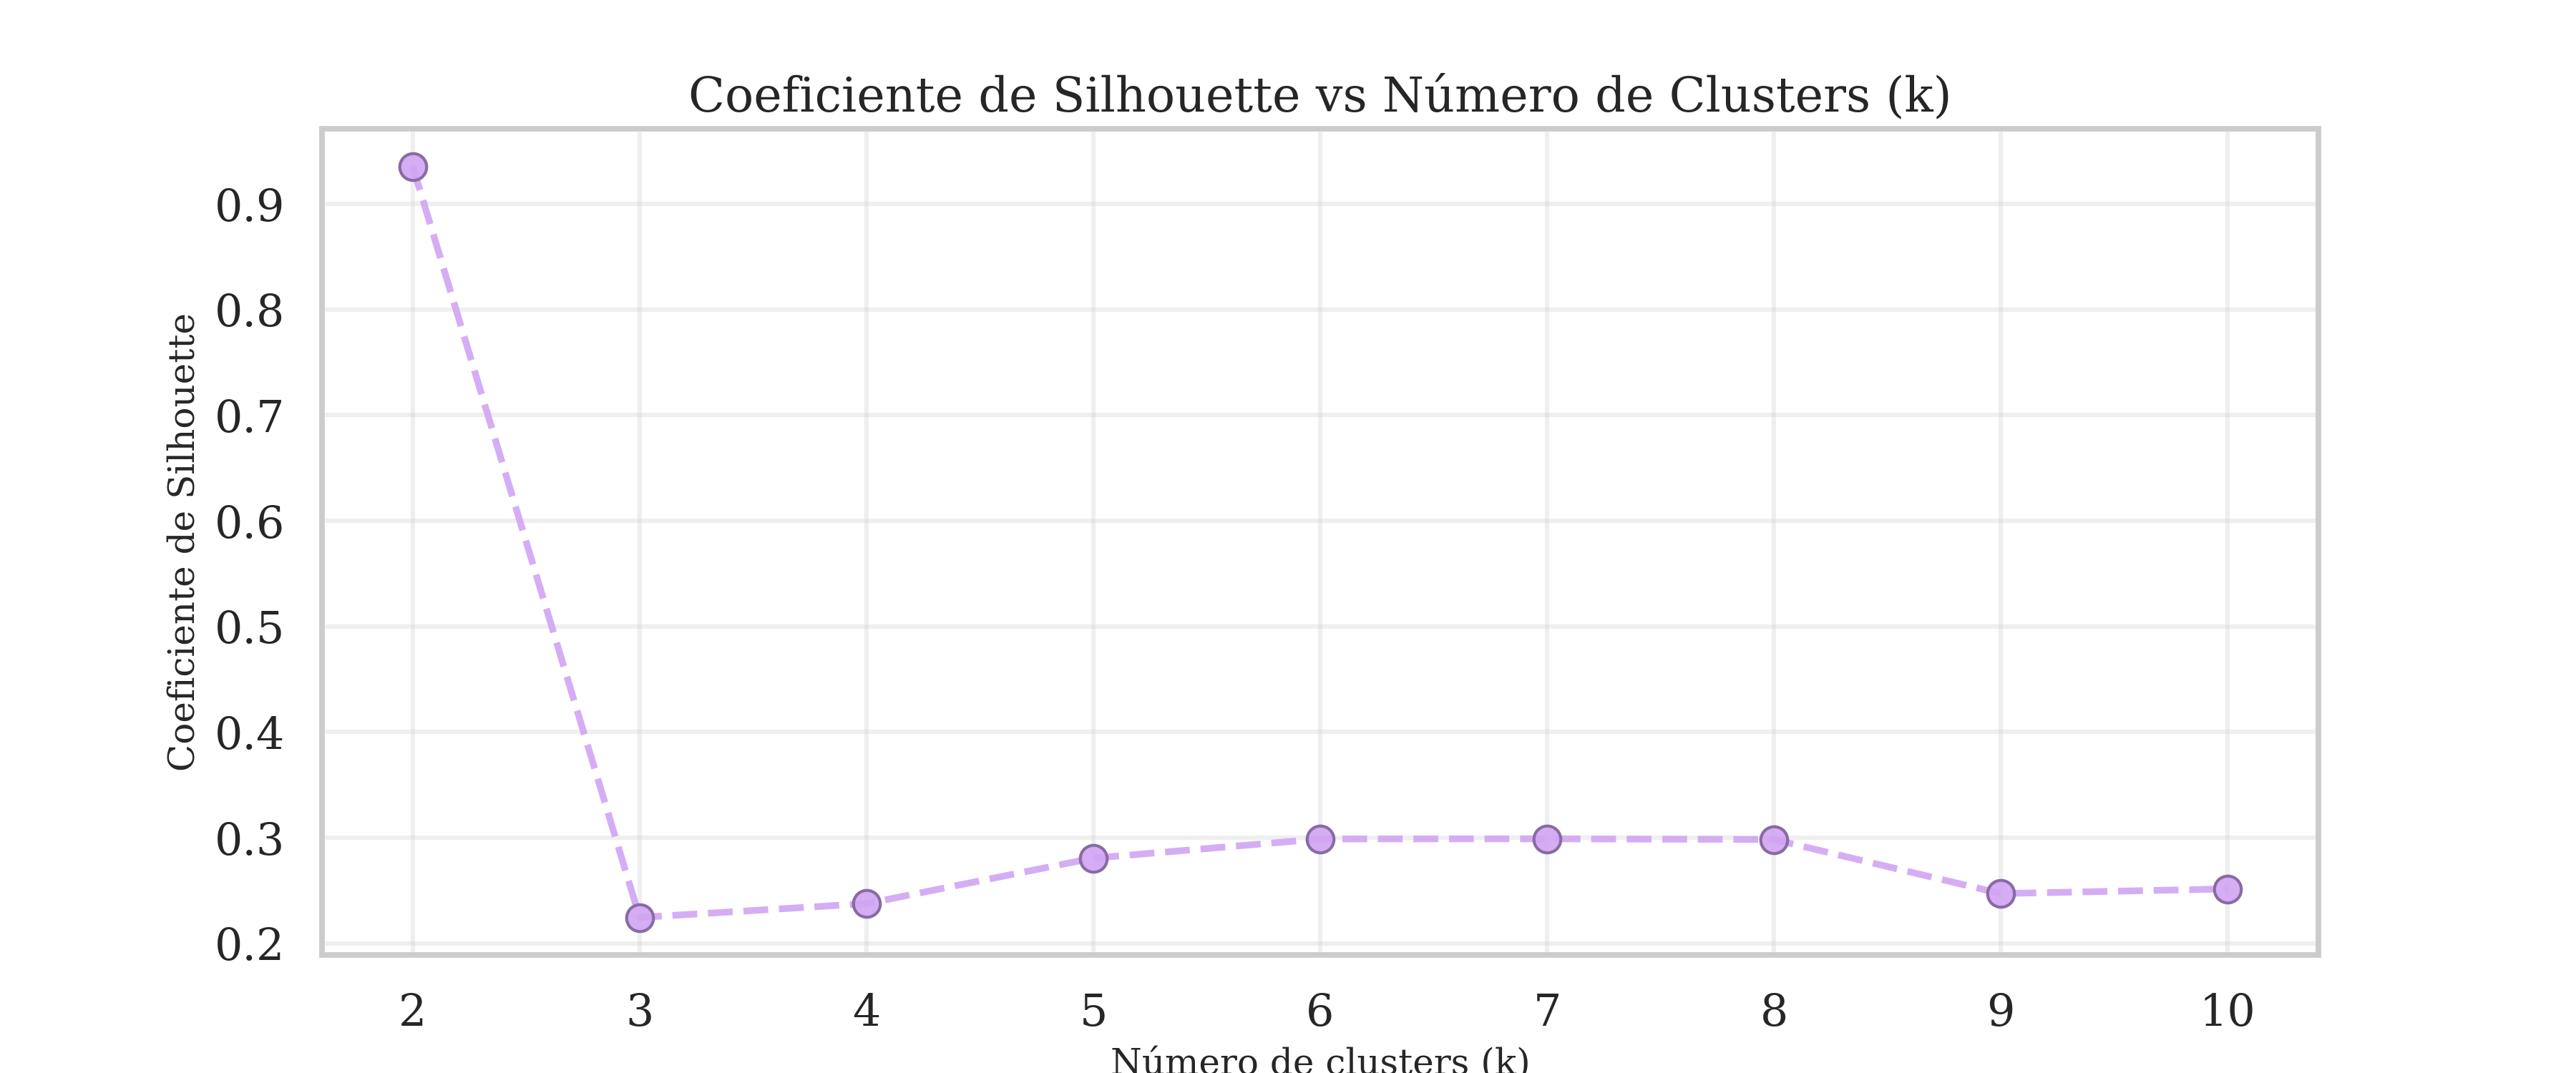
\includegraphics[width=0.87\textwidth]{silhouette_vs_k_kmeans.png}
    \caption{Coeficiente de Silhouette promedio para $k$ entre 2 y 10.}
    \label{fig:silhouette}
\end{figure}

Con base en ambos criterios y en la interpretabilidad de los perfiles resultantes, se fijó $k = 5$ como 
número de clusters para el modelo final. Las etiquetas obtenidas se incorporaron posteriormente al conjunto limpio 
original (\texttt{df\_clustering}) para formar el DataFrame \texttt{df\_resultado}, que se utiliza en la sección 
de resultados para analizar y describir en detalle los perfiles de endeudamiento correspondientes a cada cluster.

\section{Resultados}

Una vez ajustado el modelo de agrupamiento, el análisis se centró en describir los perfiles financieros de los 
cinco clusters obtenidos. Para ello se combinaron estadísticas descriptivas y visualizaciones que permiten comparar 
cada grupo en dimensiones como morosidad, endeudamiento, ingresos y actividad crediticia. Aunque no se muestran 
todas las gráficas generadas (como la proyección PCA o los boxplots), estas confirmaron que los clusters presentan 
diferencias bien definidas y coherentes con los patrones observados en el conjunto.

\subsection{Perfilamiento general de los clusters}

Como punto de partida, se calcularon las medias de las variables financieras para cada cluster, además del tamaño 
absoluto y relativo de cada grupo. La Tabla~\ref{tab:perfilamiento-clusters} organiza esta información por temas 
principales: nivel de endeudamiento, morosidad, actividad crediticia, características demográficas y dimensión de 
cada cluster. Esta estructura permite identificar diferencias globales antes de recurrir a visualizaciones más detalladas.

\begin{table}[H]
\centering
\caption{\textbf{Perfilamiento general de los clusters por temática}}
\label{tab:perfilamiento-clusters}
\small
\rowcolors{2}{lavandaClaro!30}{white}

\begin{tabular}{
    p{4.8cm}
    >{\centering\arraybackslash}p{1.4cm}
    >{\centering\arraybackslash}p{1.4cm}
    >{\centering\arraybackslash}p{1.4cm}
    >{\centering\arraybackslash}p{1.4cm}
    >{\centering\arraybackslash}p{1.4cm}
}
\toprule
\rowcolor{lavanda!40}
\textbf{Variable} & \textbf{0} & \textbf{2} & \textbf{3} & \textbf{4} & \textbf{1} \\
\midrule

\multicolumn{6}{l}{\textbf{Endeudamiento y uso de crédito}} \\
Revolving Utilization & 0.107 & 0.690 & 0.260 & 0.277 & 1.000 \\
Debt Ratio             & 131.673 & 92.730 & 37.194 & 3305.179 & 6.764 \\[4pt]

\multicolumn{6}{l}{\textbf{Morosidad (frecuencia de atrasos)}} \\
30--59 días tarde & 0.121 & 0.389 & 0.286 & 0.245 & 97.956 \\
60--89 días tarde & 0.023 & 0.226 & 0.052 & 0.050 & 97.956 \\
90+ días tarde    & 0.023 & 0.245 & 0.043 & 0.050 & 97.956 \\[4pt]

\multicolumn{6}{l}{\textbf{Actividad crediticia}} \\
Líneas abiertas              & 7.937 & 5.226 & 12.237 & 10.049 & 0.009 \\
Préstamos inmobiliarios     & 0.701 & 0.442 & 1.887 & 1.778 & 0.000 \\[4pt]

\multicolumn{6}{l}{\textbf{Ingresos y características demográficas}} \\
Ingreso mensual      & 5912.836 & 4789.837 & 9229.359 & 5124.065 & 3602.027 \\
Edad                 & 62.498 & 40.893 & 48.875 & 53.395 & 36.071 \\
Dependientes         & 0.178 & 0.664 & 1.739 & 0.400 & 0.000 \\[4pt]

\multicolumn{6}{l}{\textbf{Tamaño del cluster}} \\
Conteo (individuos)  & 58054 & 40646 & 39604 & 10861 & 225 \\
Porcentaje (\%)      & 38.861 & 27.208 & 26.510 & 7.270 & 0.151 \\

\bottomrule
\end{tabular}
\end{table}

La tabla muestra que el cluster~1 concentra valores extremos en todas las variables de 
morosidad y casi ninguna línea de crédito activa, además de representar sólo el 0.15\% de 
la población. Por este motivo, algunas visualizaciones posteriores lo excluyen para evitar 
que distorsione la escala.
\newpage
\subsection{Mapa de calor de perfiles por cluster}

El mapa de calor de la Figura~\ref{fig:heatmap-clusters} resume las medias normalizadas de cada variable en cada cluster. 
Esta visualización permite comparar rápidamente la posición relativa de cada grupo sin necesidad de analizar cada variable por separado.

\begin{figure}[H]
    \centering
    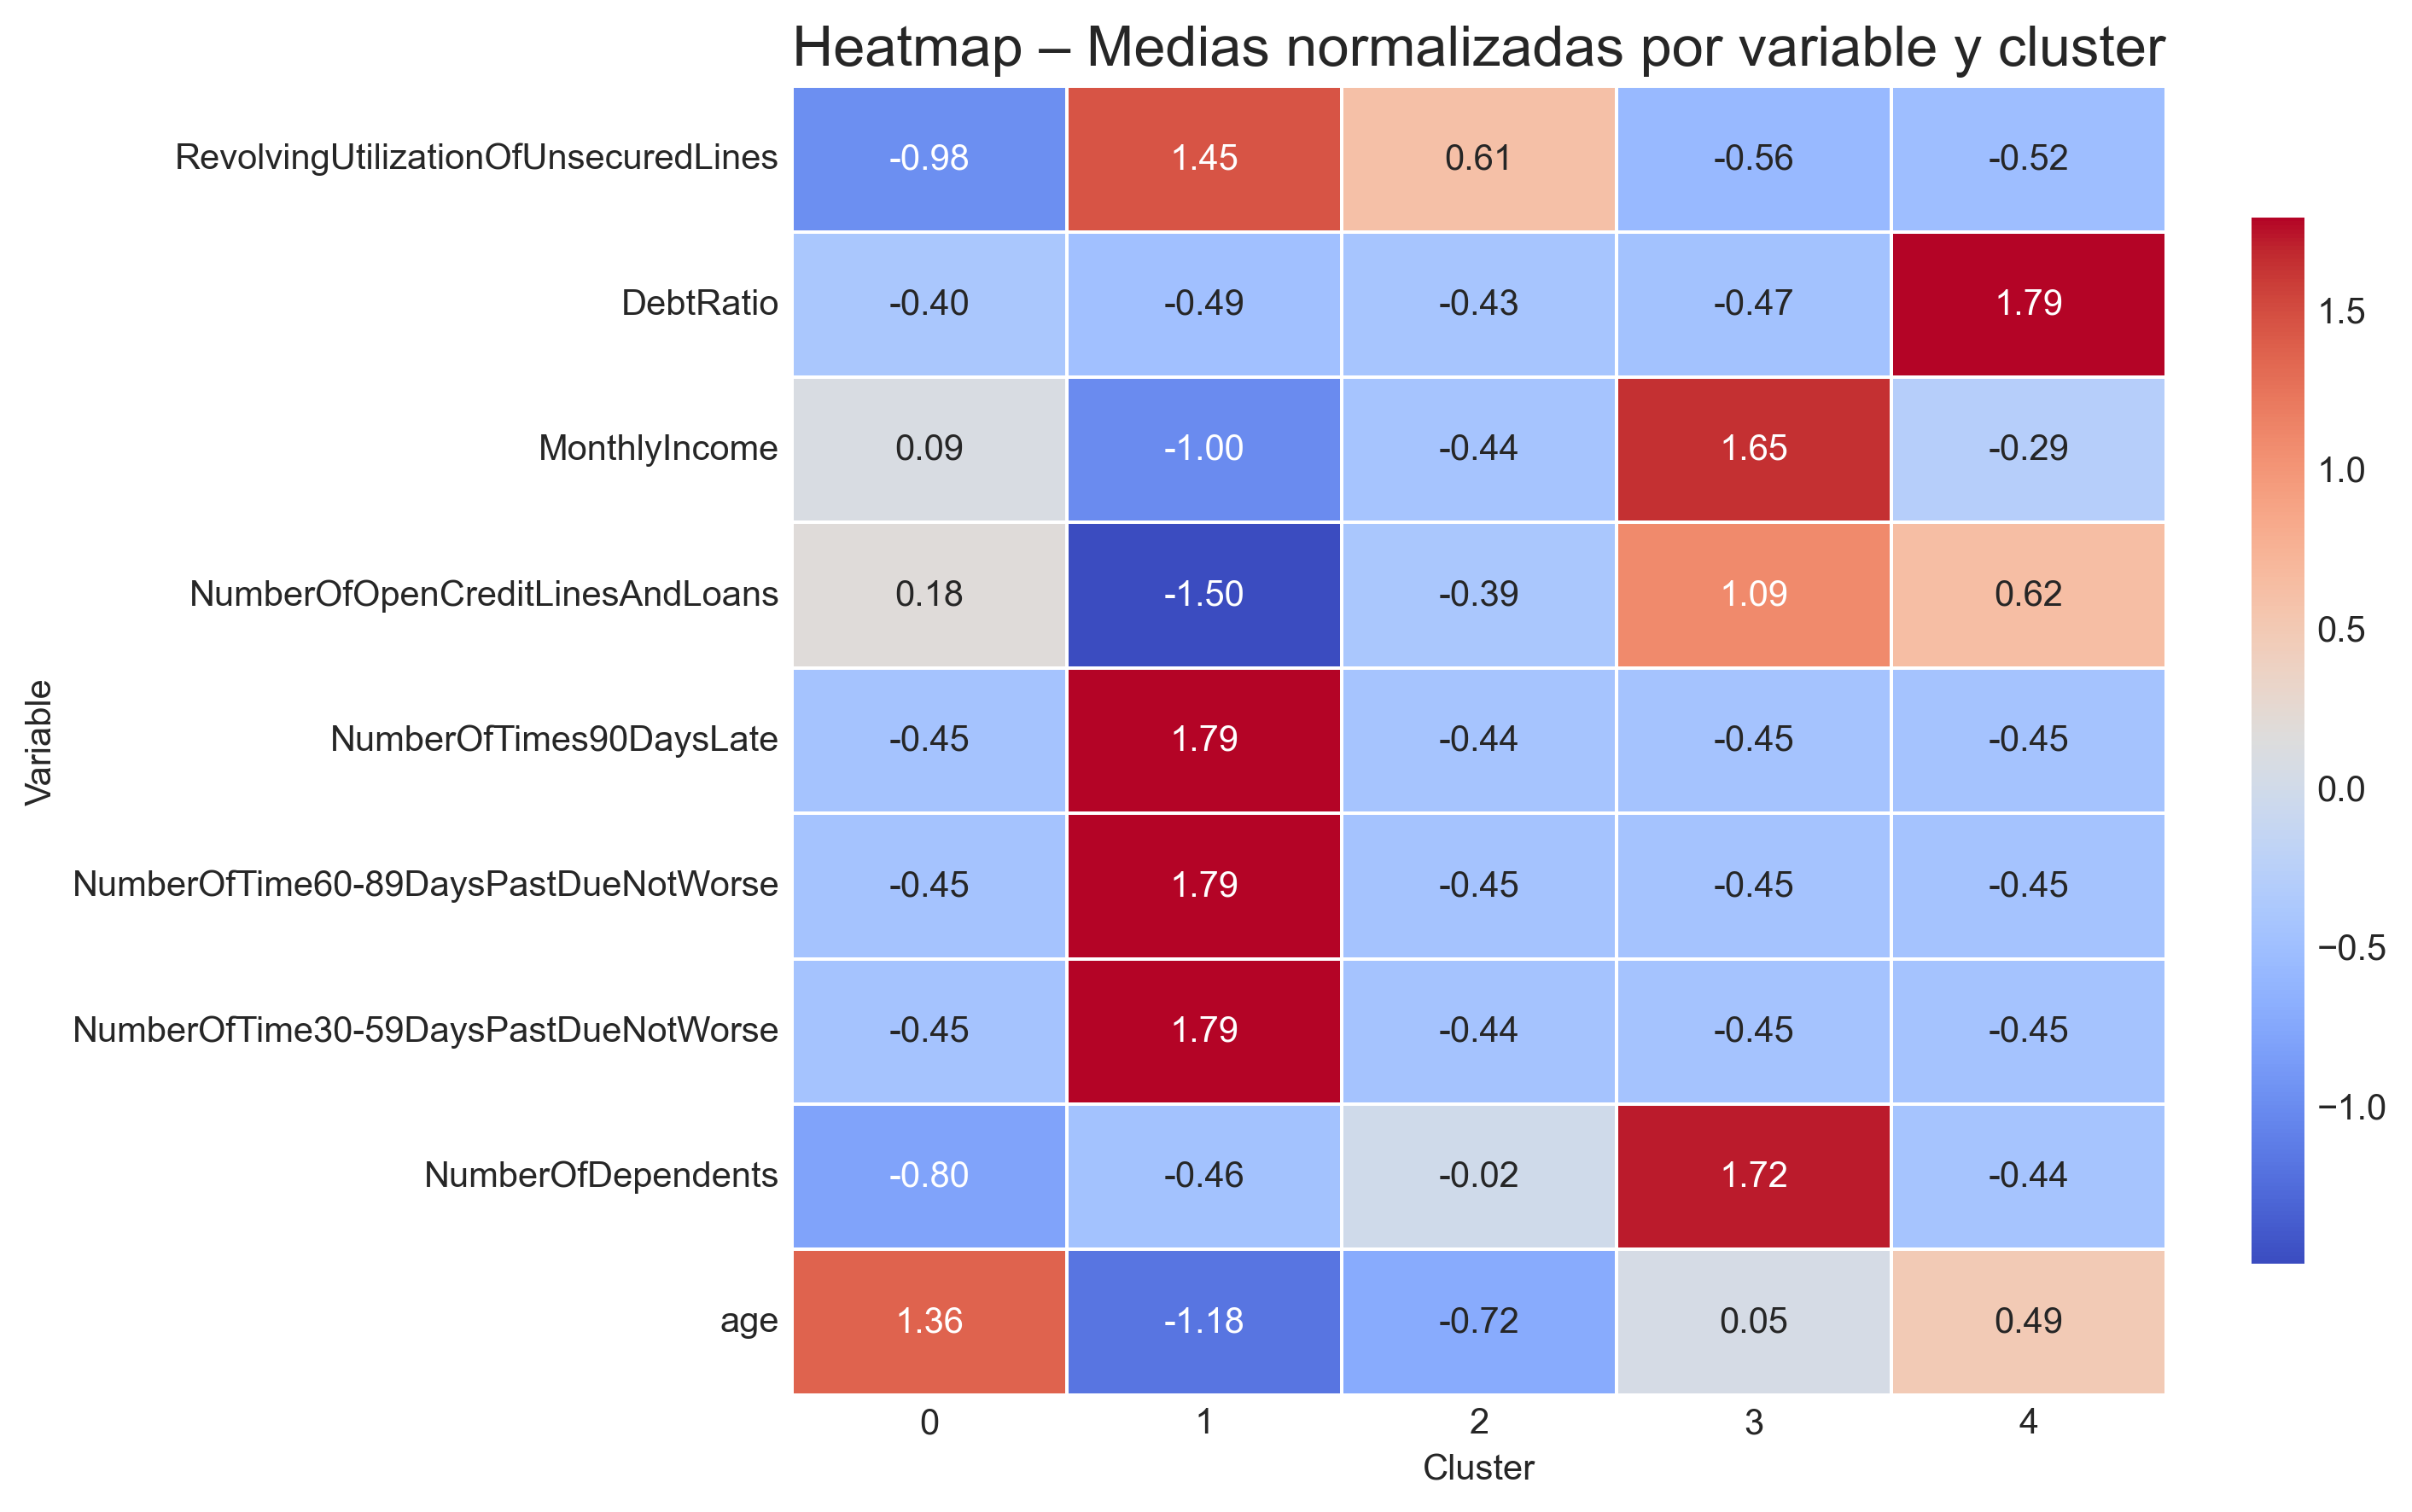
\includegraphics[width=0.88\textwidth]{heatmap_clusters.png}
    \caption{Mapa de calor de medias normalizadas (z-score) para las variables financieras según cluster.}
    \label{fig:heatmap-clusters}
\end{figure}

Lo anterior nos revela contrastes bien definidos, el cluster~0 presenta valores consistentemente bajos en morosidad y 
utilización del crédito; el cluster~3 destaca por sus altos ingresos y amplia actividad crediticia; el cluster~4 
muestra niveles muy elevados de endeudamiento; mientras que el cluster~2 combina mayor carga familiar con una 
utilización más intensa del crédito. El cluster~1 resalta de forma inmediata debido a sus valores extremos 
en todas las medidas de atraso.

\subsection{Perfilamiento global mediante gráfico de radar}

El gráfico de radar de la Figura~\ref{fig:radar-clusters} complementa al mapa de calor ofreciendo una vista 
conjunta de los perfiles. Para preservar la escala y la legibilidad, el cluster~1 se excluyó de esta representación.

\begin{figure}[H]
    \centering
    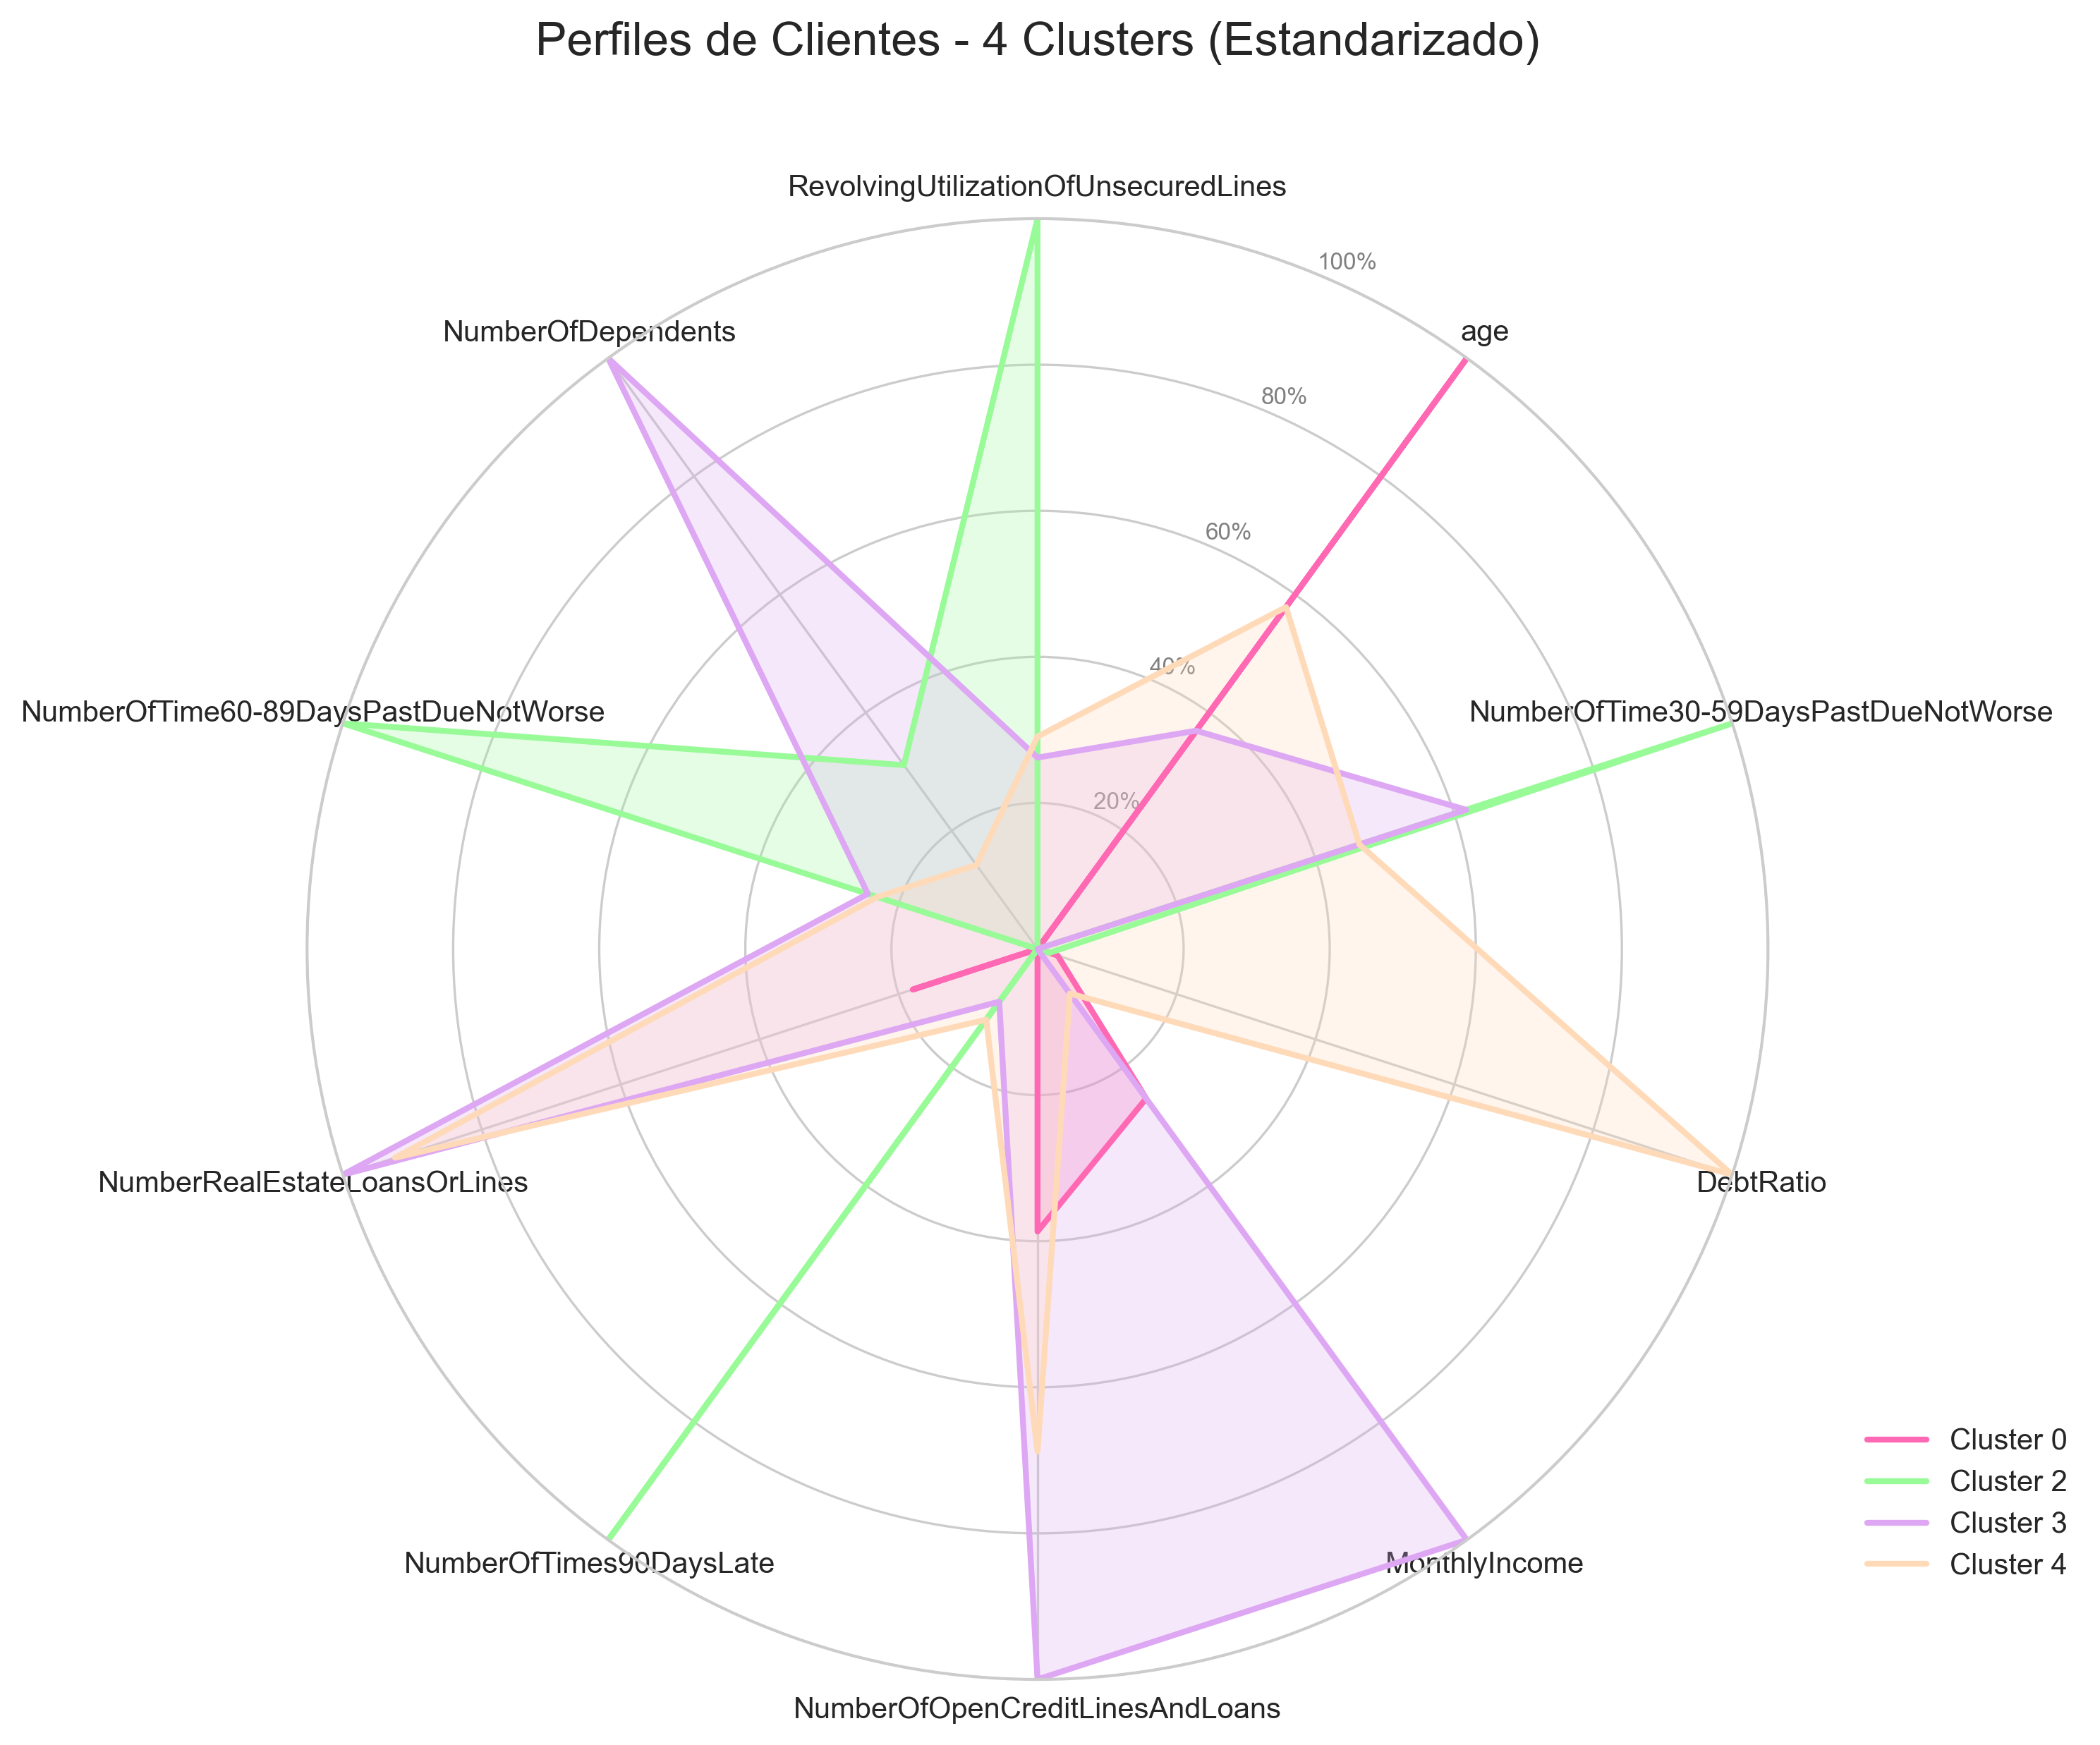
\includegraphics[width=0.80\textwidth]{segmentacion_radar_clusters.png}
    \caption{Gráfico de radar comparando las medias normalizadas de los clusters (excepto el cluster 1).}
    \label{fig:radar-clusters}
\end{figure}

Aquí se aprecia la “forma” distintiva de cada perfil: el cluster~0 reúne valores bajos y estables; el cluster~3 
sobresale en ingreso y actividad crediticia; el cluster~2 se expande en dimensiones asociadas a carga familiar y 
uso del crédito; y el cluster~4 se distingue por su fuerte componente de endeudamiento. A diferencia del mapa de 
calor, el radar permite observar cómo cada cluster distribuye su intensidad relativa entre las variables.

\subsection{Interpretación de los clusters}

A partir del perfilamiento cuantitativo y de las visualizaciones generadas, es posible describir con claridad las 
características distintivas de cada uno de los grupos identificados. Los clusters representan perfiles financieros 
bien diferenciados, que reflejan patrones concretos de utilización del crédito, estabilidad económica y comportamiento 
de pago.

\textbf{Cluster 0: Perfil estable y conservador.}  

Este grupo agrupa al porcentaje más grande de la población (38.9\%). Se caracteriza por una utilización muy baja 
del crédito rotativo, niveles prácticamente nulos de morosidad y una edad promedio elevada. Además, sus ingresos 
se encuentran en niveles moderados y el número de líneas de crédito abiertas es relativamente bajo. Todo apunta 
a un perfil de clientes prudentes, con un comportamiento crediticio estable y sin señales de riesgo significativo.

\textbf{Cluster 2: Uso intensivo del crédito y mayor vulnerabilidad.} 

Los individuos de este cluster presentan una utilización del crédito rotativo notablemente alta, mayores niveles 
de morosidad (en comparación con los clusters estables) y una proporción importante de dependientes. La edad 
promedio es menor y los ingresos son moderados, lo que sugiere una etapa más temprana en la vida financiera 
con una carga económica elevada. Este grupo refleja un perfil más vulnerable ante variaciones en ingresos o 
gastos, con riesgo de deterioro futuro.

\textbf{Cluster 3: Actividad crediticia elevada y mayor capacidad económica.}  

Este cluster destaca por tener los ingresos más altos de la población y un número considerable de líneas 
de crédito, incluidas líneas inmobiliarias. La morosidad es baja y la utilización del crédito rotativo es 
moderada, lo que indica control y diversificación financiera. Corresponde a clientes con una posición 
económica más sólida y un nivel alto de actividad en el sistema financiero.

\textbf{Cluster 4: Perfil sobreendeudado.}  

El rasgo más notable de este cluster es su \textit{DebtRatio} extremadamente elevado, indicando que una 
fracción muy alta del ingreso declarado se destina al pago de deudas y gastos. Aunque los indicadores de 
morosidad no son tan extremos como en el cluster 1, sí muestra señales claras de estrés financiero. La 
actividad crediticia es relativamente alta, pero los ingresos se mantienen en niveles medios, lo que 
contribuye al sobreendeudamiento observado.

\textbf{Cluster 1: Morosidad extrema y actividad crediticia mínima (outlier).} 

Este grupo, el más pequeño de todos (0.15\%), presenta valores extraordinariamente altos en todos 
los indicadores de morosidad (30--59, 60--89 y 90+ días de atraso), así como ingresos bajos y casi 
ninguna línea de crédito activa. Su comportamiento lo distingue de manera clara del resto de la población, 
por lo que fue tratado como un outlier en algunas visualizaciones. Representa un perfil de riesgo máximo, 
asociado a incumplimientos continuos y ausencia de participación estable en el sistema crediticio.

En conjunto, estos cinco perfiles muestran la diversidad de comportamientos financieros presentes en 
la población analizada y permiten interpretar la segmentación no supervisada de manera significativa. 
Cada cluster refleja un tipo de cliente distinto, con condiciones económicas y hábitos crediticios 
particulares, lo cual es útil para análisis posteriores relacionados con riesgo, solvencia o posibles 
estrategias de intervención.

\section{Discusión}

Los resultados obtenidos permiten apreciar que el proceso de segmentación identifica patrones financieros 
coherentes y consistentes con dinámicas reales de endeudamiento y comportamiento crediticio. La estructura 
revelada por los cinco clusters no surge únicamente de diferencias marginales, sino de combinaciones claras 
de variables que representan dimensiones económicas fundamentales: estabilidad, capacidad de pago, intensidad 
crediticia y riesgo de incumplimiento.

Una observación relevante es que los perfiles no se distribuyen de manera uniforme dentro de la población. 
La mayor parte de los individuos pertenece a clusters con comportamiento relativamente estable, mientras 
que los grupos más vulnerables o con señales de sobreendeudamiento representan proporciones menores. Esto 
sugiere que el conjunto de clientes no está compuesto mayoritariamente por usuarios de riesgo extremo, 
sino por personas con hábitos financieros diversos en distintos grados de madurez y estabilidad económica.

Otro punto importante es la presencia del cluster~1, cuyo comportamiento atípico evidencia que la población 
contiene un subconjunto de individuos con dificultades severas y sostenidas en su historial de pago. Este grupo, 
si bien minoritario, tiene un impacto relevante para cualquier análisis de riesgo, pues concentra valores 
extremos que en muchos casos distorsionan representaciones visuales o medidas globales. Su identificación 
confirma la utilidad del aprendizaje no supervisado para detectar segmentos que no serían visibles mediante análisis 
unidimensionales.

Finalmente, la coexistencia de clusters con características contrastantes por ejemplo, el grupo de 
alto ingreso y alta actividad crediticia frente al grupo sobreendeudado, muestra que la heterogeneidad 
del conjunto no se explica únicamente por el nivel de ingreso, sino por la interacción entre múltiples 
dimensiones financieras. En este sentido, el uso combinado de PCA y K-Means permitió capturar la estructura 
del conjunto con una representación clara y útil para su interpretación.

\section{Conclusiones, limitaciones y supuestos}

El análisis realizado permitió construir una segmentación no supervisada de clientes basada en características 
financieras de uso del crédito, morosidad, endeudamiento e ingreso. La metodología empleada, que combina un 
preprocesamiento cuidadoso, una reducción de dimensionalidad mediante PCA y un modelo de agrupamiento tipo K-Means, 
proporcionó cinco perfiles claramente diferenciados. Estos perfiles ofrecen una visión estructurada de la población 
y permiten identificar comportamientos financieros que van desde la estabilidad y el uso prudente del crédito hasta 
el sobreendeudamiento y la morosidad extrema.

Una conclusión importante es que la estructura identificada no depende de una única variable, sino de la interacción 
entre múltiples dimensiones financieras. Esto refuerza la utilidad de los métodos no supervisados para descubrir 
patrones que no son evidentes mediante análisis directos o modelos univariados. Al mismo tiempo, la segmentación 
obtenida puede servir como base para análisis posteriores, por ejemplo, estudios de riesgo crediticio, estrategias de 
intervención o modelos supervisados que utilicen los clusters como características adicionales.

\subsection*{Limitaciones}

A pesar de los resultados obtenidos, el estudio presenta algunas limitaciones que deben considerarse:

\begin{itemize}
    \item \textbf{Calidad y distribución de los datos.} El conjunto contiene variables con fuerte asimetría y valores 
    extremos que, aunque suavizados mediante winsorización, pueden influir en la estabilidad de los componentes principales y los centroides del clustering.
    \item \textbf{Ausencia de información temporal.} Los datos representan un corte transversal; no es posible analizar la evolución financiera de los 
    individuos ni inferir transiciones entre perfiles.
    \item \textbf{Dependencia del método elegido.} K-Means asume clusters esféricos y separados principalmente por distancia euclidiana. 
    Otros métodos (GMM, clustering jerárquico o DBSCAN) podrían revelar estructuras diferentes.
    \item \textbf{Tamaño altamente desigual de los grupos.} La presencia de un cluster extremadamente pequeño pero muy atípico plantea desafíos interpretativos y 
    puede requerir un tratamiento especial en aplicaciones reales de riesgo.
\end{itemize}

\subsection*{Supuestos}

El análisis se desarrolló bajo varios supuestos:

\begin{itemize}
    \item El preprocesamiento aplicado (imputación, truncamiento y estandarización) conserva de manera adecuada la estructura financiera del conjunto.
    \item Los componentes principales utilizados capturan la mayor parte de la variabilidad relevante para el agrupamiento.
    \item La elección de $k=5$, si bien guiada por criterios estadísticos, también responde a consideraciones interpretativas y prácticas.
    \item Las medias dentro de cada cluster son representativas de su perfil general, aun cuando algunos grupos presenten alta variabilidad interna.
\end{itemize}

En conjunto, el estudio ofrece una segmentación robusta y útil, con una interpretación clara y sustento estadístico. Sin embargo, sus conclusiones deben entenderse dentro del marco de las decisiones metodológicas y los supuestos adoptados, lo que abre la puerta a futuras extensiones, refinamientos o comparaciones con otros enfoques de análisis.


\section{Referencias}

\begin{itemize}[leftmargin=1.2cm]

\item Everitt, B., Landau, S., Leese, M., \& Stahl, D. (2011). \textit{Cluster Analysis} (5th ed.). Wiley.

\item Jain, A. K. (2010). Data clustering: 50 years beyond K-means. \textit{Pattern Recognition Letters}, 31(8), 651–666.

\item Jolliffe, I. T. (2002). \textit{Principal Component Analysis} (2nd ed.). Springer.

\item Kaggle. (2011). \textit{Give Me Some Credit - Credit Risk Dataset}. Recuperado de: \url{https://www.kaggle.com/c/GiveMeSomeCredit}

\item Lloyd, S. (1982). Least squares quantization in PCM. \textit{IEEE Transactions on Information Theory}, 28(2), 129–137.

\end{itemize}

\end{document}


